\documentclass{hertieteaching}
\addbibresource{/Users/wlowe/Bibliography/zotero.bib}

\usepackage{relsize}

\title{More scaling}

\begin{document}

{\setbeamertemplate{footline}{}
\begin{frame}
\maketitle
\end{frame}}
\addtocounter{page}{-1}

\begin{frame}{Plan}
\begin{itemize}
  \item Interpretation
  \item Multidimensional models
  \item Comparisons 
  \item Connections to other methods
\end{itemize}

\end{frame}

\begin{frame}{The model (ml version)}

\begin{columns}[T,onlytextwidth]
\column{0.5\textwidth}

\begin{center}
\begin{tikzpicture}
\node(theta) at (3,0)[var,label=right:$\theta$]{};
\node(W) at (1.5,0)[var,label=below:$W$]{};
\node(beta) at (0,0)[var,label=left:$\beta$]{};
\node(alpha) at (3,1)[var,label=right:$\alpha$]{};
\node(psi) at (0,-1)[var,label=left:$\psi$]{};
\draw(theta) -- (W);
\draw(beta) -- (W);
\draw(psi) -- (W);
\draw(alpha) -- (W);
\draw(-1,-1.5) rectangle (2.5,1)[gray];
\node(labv) at (-1.2,-1.4)  []{{\color{gray}\small V}};
\draw(0.5,-1) rectangle (4,1.5)[gray];
\node(labn) at (4.2,-0.9)  []{{\color{gray}\small N}};
\end{tikzpicture}
\end{center}

\medskip
\smallskip
$$
\log C_\mathit{ij} = \alpha_i + \psi_j + \theta_i \beta_j
$$

\column{0.05\textwidth}
\column{0.45\textwidth}
Model fitting by `coordinate ascent' \parencite{Goodman1979}
\begin{itemize}
  \item[0.] Guess $\theta$ and $\alpha$
  \item[1.] Fit each $\beta_j$ (as slope) and $\psi_j$ (as intercept) as a Poisson regression with offset $\alpha$ and `covariates' $\theta$
  \item[2.] Fit each $\theta_i$ (as slope) and $\alpha_i$ (as intercept) in a  Poisson regression with offset $\psi$ and `covariates' $\beta$
  \item[3.] If the likelihood is not yet maximized, go to step 2. 
\end{itemize}
Slow, but reasonably reliable.
\end{columns}

\end{frame}


\begin{frame}{Unidimensionality}

What is this $\theta$ anyway?
\begin{itemize}
  \item Whatever fits the data best. You have to interpret them
\end{itemize}

Last week's `spatial talking' implies that
\begin{itemize}
  \item Document positions are an average of the $\beta$s of the words in them (and word positions are an average of the documents they appear in)
  \item So if we can interpret the $\beta$s as a substantive scale, we know that the dimension is
\end{itemize}
\pause
Not everything has to be a dimension
\begin{itemize}
  \item but it does for a scaling model!
\end{itemize}
Difficult cases:
\begin{itemize}
  \item Populism and anti-system parties. Are they well understood as ideological?
  \item Government and opposition. Naturally polar but not necessarily ideologically so
\end{itemize}


\end{frame}

\begin{frame}{Unidimensionality}
Related questions
\begin{itemize}
  \item How do we know that positions are only one dimension?
  \item How to get positions on a \textit{specific} policy issue?
\end{itemize}

\pause

Possibilities, in order of directness
\begin{itemize}
\item Select vocabulary that is on topic \parencite[e.g. in sentiment analysis;][]{Proksch.etal2019}
\item Use topic counts instead of words \parencite[e.g. RILE;][]{Budge.etal1987} 
\item Scale only on-topic segments of the each document \parencite{Slapin.Proksch2008}
\item Learn $\beta$ from (a subset of) known `reference' documents \parencite[`Wordscores';][]{Laver.etal2003}
\item Trust institutional or strategic context to constrain to one dimension \parencite{Baerg.Lowe2020}
\end{itemize}

%All of these allow our model assumptions to be closer to true

\end{frame}

\begin{frame}{Oops}

\begin{columns}[T,onlytextwidth]
\column{0.6\textwidth}
{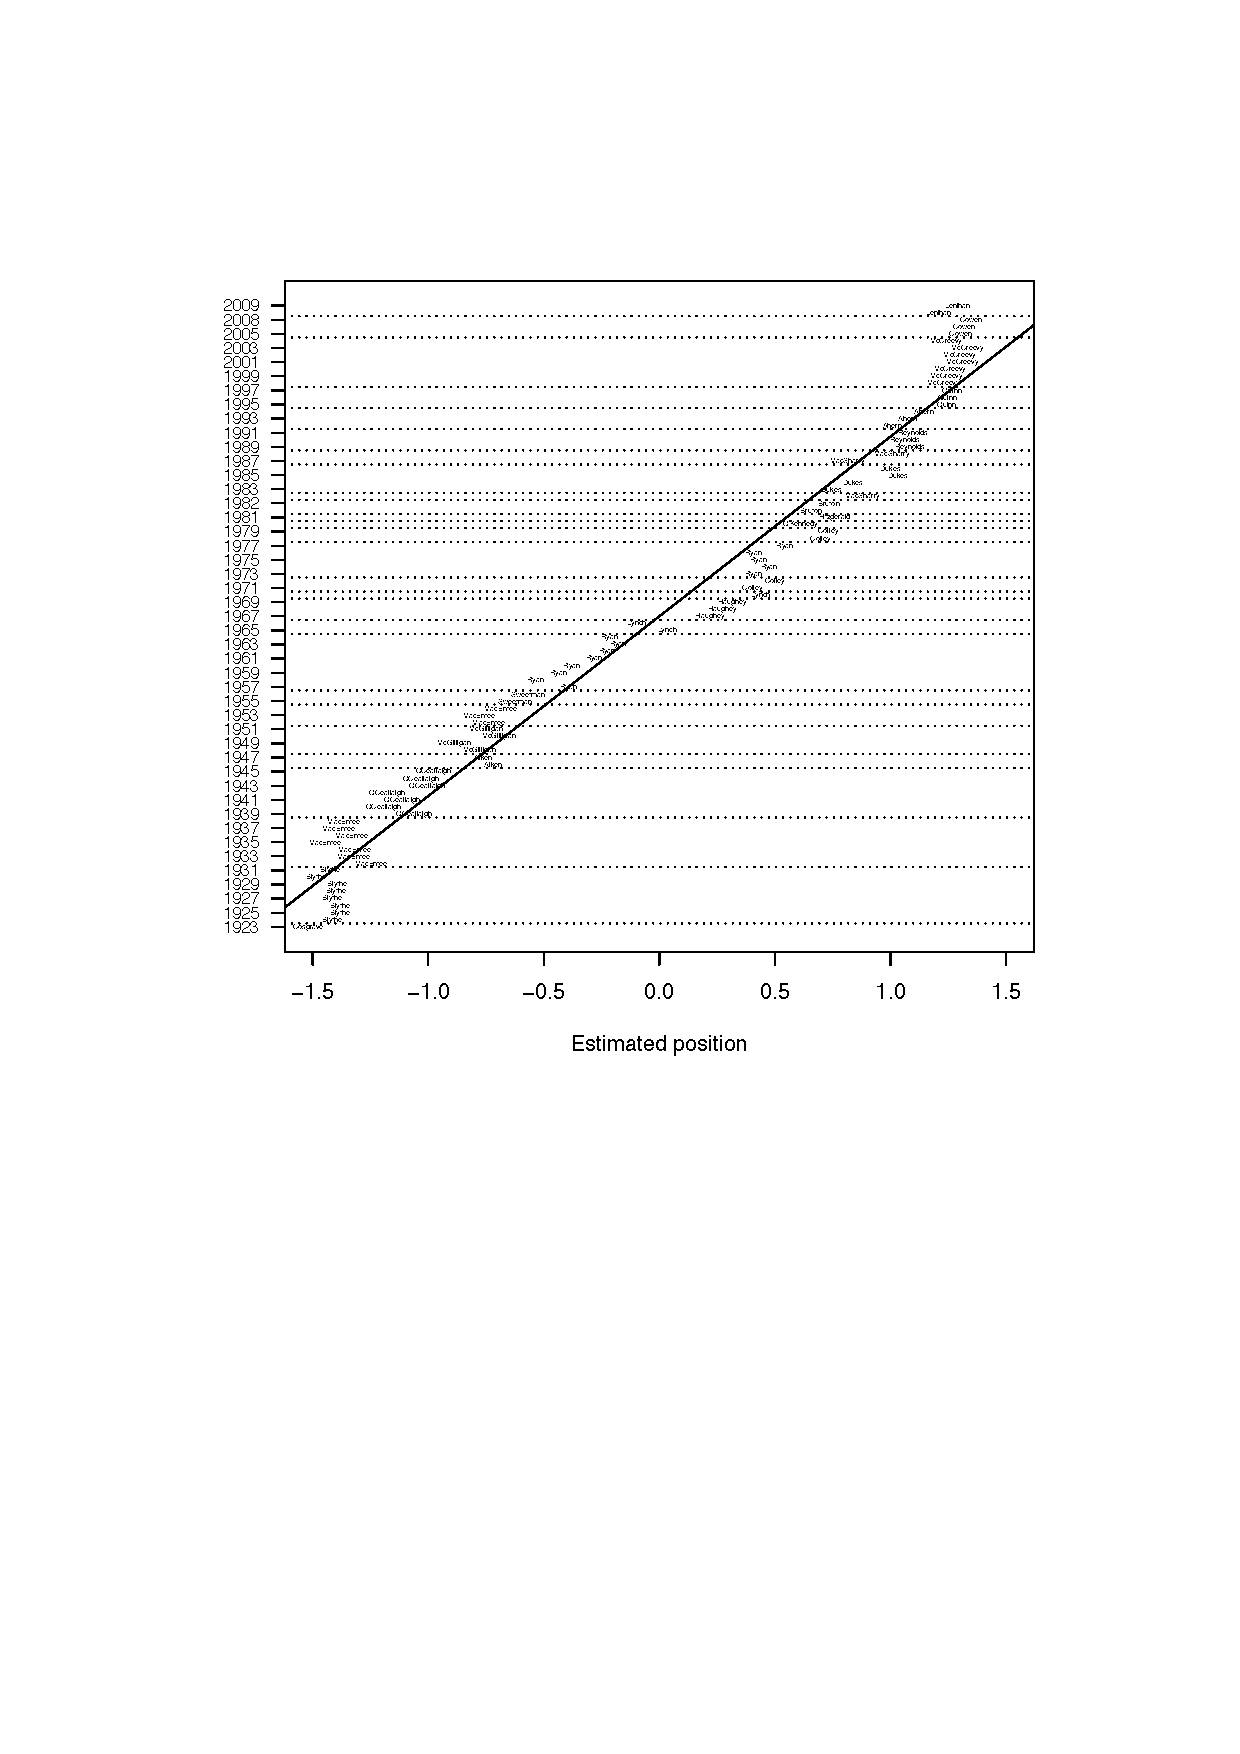
\includegraphics[scale=0.55]{pictures/HandMfig2}}
\column{0.4\textwidth}
\medskip
\textit{All} the budget speeches in independent Irish history,
scaled.

\begin{itemize}
  \item Budgets are about spending money on things
  \item Those things change over time
  \item The model cannot know
\end{itemize}
\medskip
\pause
Possible fix
\begin{itemize}
  \item Choose a subset of stable vocabulary \parencite{Proksch.Slapin2009a}
\end{itemize}
\end{columns}
\end{frame}

\begin{frame}{Vocabulary decisions}
\medskip
\centerline{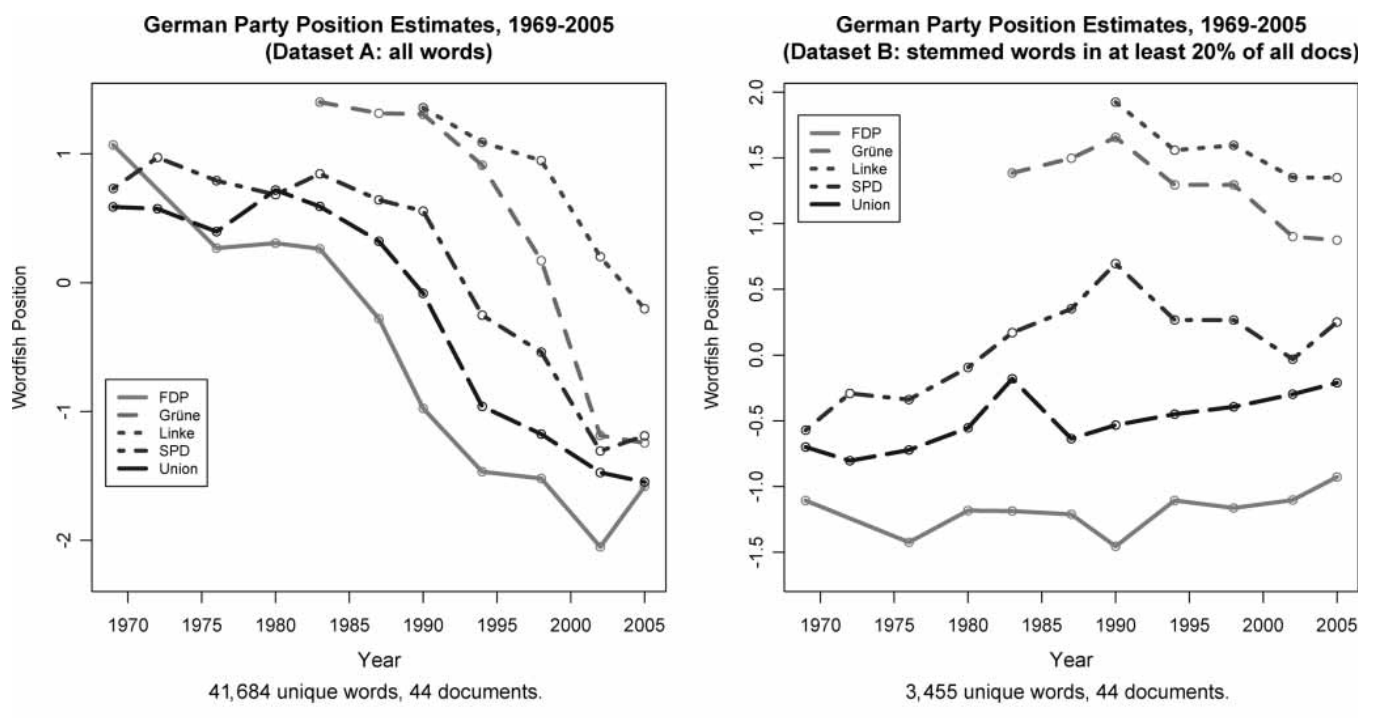
\includegraphics[scale=0.55]{pictures/proksch-de-comparable-1}}
\end{frame}

\begin{frame}{Vocabulary decisions}
\medskip
\centerline{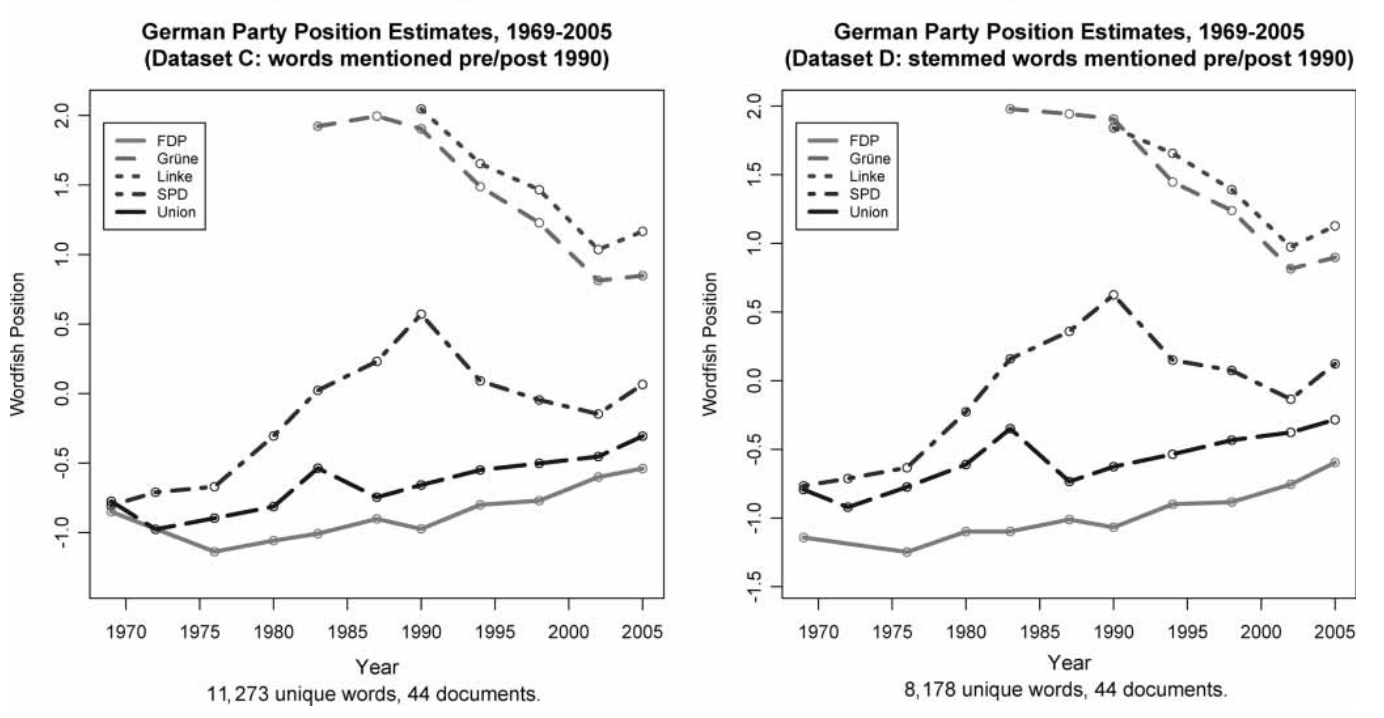
\includegraphics[scale=0.55]{pictures/proksch-de-comparable-2}}
\end{frame}


\begin{frame}{Wordscores}

Wordscores is an early approach to topic-specific unidimensional scaling \parencite{Laver.etal2003}
\begin{itemize}
  \item[0.] Assert the positions of $R$ reference documents $\theta_1 \ldots \theta_R$
  \item[1.] Using only these, estimate $\beta$ (there are no $\psi$s)
  \item[2.] Estimate each remaining $\theta$s as the average of the $\beta$s of its words
  $$
  \hat{\theta}_i ~=~ \frac{1}{N} \sum^{N}_i \beta_\mathit{v[i]} ~=~ \sum^{V}_{v} \beta_v F(v \mid \text{document } i) 
  $$
\end{itemize}

\pause
Why does this work (when it does work?)

Intuition:
\begin{itemize}
  \item Variation across $\theta_1 \ldots \theta_R$ defines the dimension
  \item When word $v$ varies a lot over documents with similar $\theta$s then $\beta_v$ must be small because it shouldn't matter to the doesn't to $\hat{\theta}$ 
  \item \ldots Profit?
\end{itemize}

\end{frame}

\begin{frame}{The model (geometrical version)}

We can also a lot of dimensions at once
\begin{itemize}
  \item Not straightforward with maximum likelihood
  \item Very easy if we move to least squares
\end{itemize}

Linear probability model: 
\begin{itemize}
  \item Previously we modeled (the log of) $E[C_\mathit{ij}]$
  \item This time we will model the proportion of corpus's counts that are document $i$ using word $j$
$$
P_\mathit{ij} = C_\mathit{ij} / N
$$
\end{itemize}
If we compute the marginal proportions
\begin{align*}
P_i & = \sum_{j} P_\mathit{ij} & 
P_j & = \sum_{i} P_\mathit{ij} 	
\end{align*}
then the probability of seeing word $j$ in document $i$ `by chance' is
$P_i P_j$ (the `independence model')

\end{frame}
\begin{frame}{The model (geometrical version)}

Define a normalized \textit{residual}
$$ 
R_\mathit{ij} = \frac{P_\mathit{ij} - P_i P_j}{\sqrt{P_i P_j}}
$$
decompose it by SVD to get orthogonal `positions'
$$ 
R = U\Sigma V^{T}
$$
Identify the first $k$ columns of $U$ as $\theta_1\ldots \theta_K$ and
the top $k$ columns of $V$ as $\beta_1\ldots \beta_K$
\bigskip
\pause
$$
P_{ij} ~\approx~ P_{i}\,P_{j}\,\left(1 + \sum^{K}_k \theta^{(k)}_i \sigma^{(k)} \beta^{(k)}_j\right)
$$
This is \textit{correspondence analysis} \parencite{Benzecri1992,Greenacre2007}

\end{frame}
\begin{frame}{Compare and contrast}

This tends to be very close to the ML version of out model
\begin{itemize}
  \item But we get $K$ dimensional positions 
  \item But no standard errors, since it's a geometrical model
\end{itemize}

Why is it similar? Because
$$
\log\left( 1 + \sum^{K}_k \theta^{(k)}_i \sigma^{(k)} \beta^{(k)}_j\right) ~\approx~ \sum^{K} \theta^{(k)}_i \sigma^{(k)} \beta^{(k)}_j
$$
when there there is smallish amounts of positioning happening.\footnote{Note: the left hand side parameters are from CA and the right hand side are from Association/Wordfish model. I just haven't distinguished them in the notation because I am a bad person.}

\end{frame}

\begin{frame}{Multidimensional positions}

\begin{columns}[T,onlytextwidth]
\column{0.5\textwidth}
\bigskip
\bigskip
\begin{center}
\begin{tikzpicture}
\node(theta) at (3,0)[var,label=right:$\theta$]{};
\node(W) at (1.5,0)[var,label=below:$W$]{};
\node(beta) at (0,0)[var,label=left:$\beta$]{};
\node(alpha) at (3,1)[var,label=right:$\alpha$]{};
\node(psi) at (0,-1)[var,label=left:$\psi$]{};
\draw(theta) -- (W);
\draw(beta) -- (W);
\draw(psi) -- (W);
\draw(alpha) -- (W);
\draw(-1,-1.5) rectangle (2.5,1)[gray];
\node(labv) at (-1.2,-1.4)  []{{\color{gray}\small V}};
\draw(0.5,-1) rectangle (4,1.5)[gray];
\node(labn) at (4.2,-0.9)  []{{\color{gray}\small N}};
\end{tikzpicture}
\end{center}

\medskip
\smallskip
$$
\log C_\mathit{ij} = \alpha_i + \psi_j + \theta_i \beta_j
$$

\column{0.05\textwidth}
\column{0.45\textwidth}

\begin{center}
\begin{tikzpicture}
\node(theta) at (3,0)[var,label=right:$\theta^{(1)}$]{};
\node(theta2) at (3,-0.5)[var,label=right:$\theta^{(2)}$]{};
\node(W) at (1.5,0)[var,label=below:$W$]{};
\node(beta) at (0,0)[var,label=left:$\beta^{(1)}$]{};
\node(beta2) at (0,0.5)[var,label=left:$\beta^{(2)}$]{};
\node(alpha) at (3,1)[var,label=right:$\alpha$]{};
\node(psi) at (0,-1)[var,label=left:$\psi$]{};
\node(sigma) at (1.5, 2)[var,label=left:$\sigma$]{};
\draw(theta) -- (W);
\draw(theta2) -- (W);
\draw(beta) -- (W);
\draw(beta2) -- (W);
\draw(psi) -- (W);
\draw(alpha) -- (W);
\draw(sigma) -- (W);
\draw(-1,-1.5) rectangle (2.5,1)[gray];
\node(labv) at (-1.2,-1.4)  []{{\color{gray}\small V}};
\draw(0.5,-1) rectangle (4,1.5)[gray];
\node(labn) at (4.2,-0.9)  []{{\color{gray}\small N}};
\end{tikzpicture}
\end{center}

$$
\log C_\mathit{ij} = \alpha_i + \psi_j + \sum_k \theta^{(k)}_i \sigma^{(k)}\beta^{(k)}_j 
$$
\end{columns}

\end{frame}



%%%%%%%%%%%%%%%%%%%%%%%%%%%%%
\begin{frame}{Partying in 2 dimensions}

\centerline{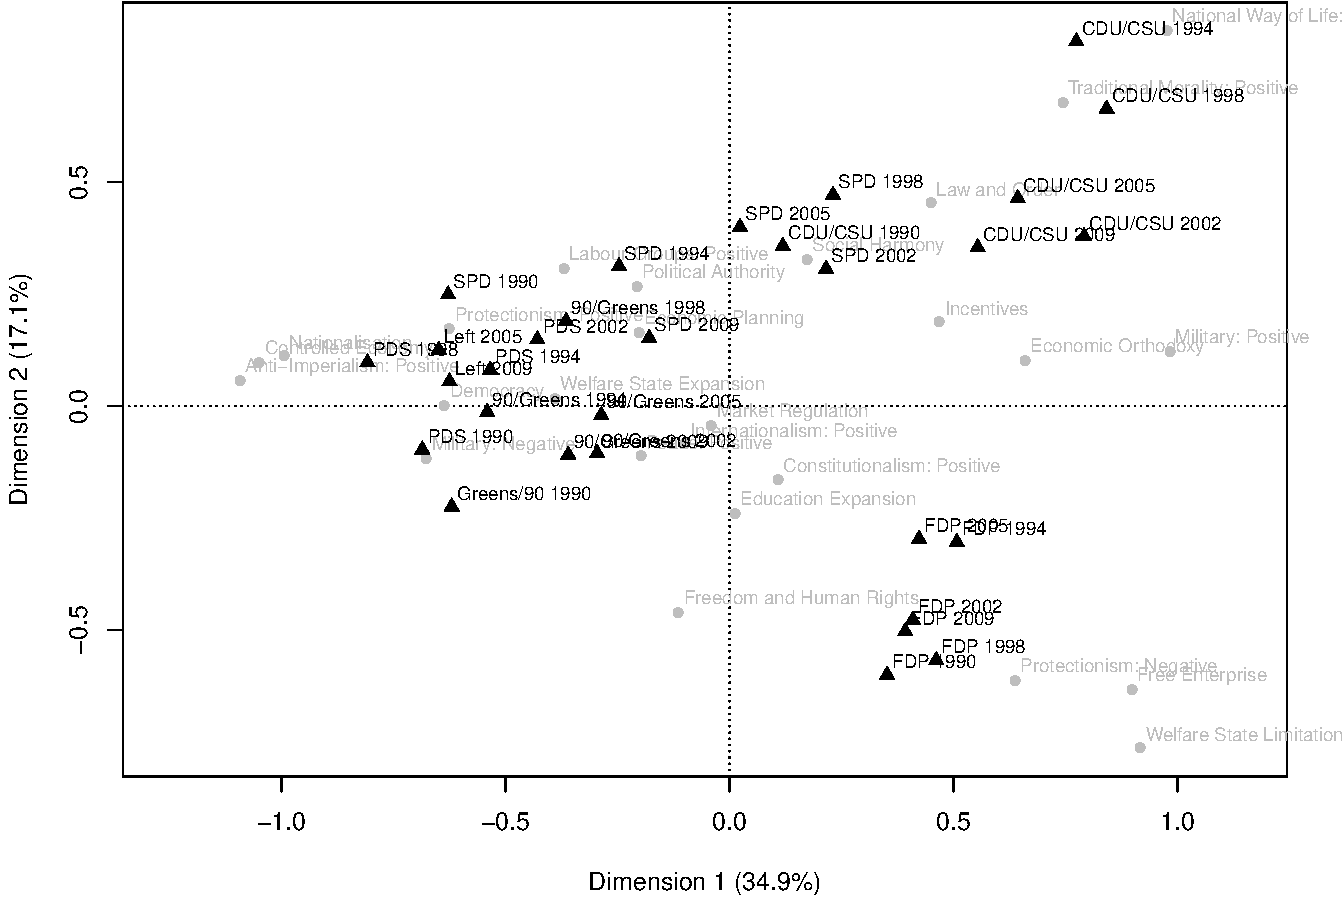
\includegraphics[scale=0.5]{pictures/grey-just-rile-crop}}

\end{frame}
\begin{frame}{Life skills}

How to read a biplot:
\begin{itemize}
  \item Documents points are closer when using words/topics similarly
  \item Words points are closer with \textit{similar} document profiles
  \item 0,0: a document or word/topic used exactly as often as we would expect by chance
  \item Document vector: arrow from 0,0 to a document point
  \item Word/topic vector: arrow from 0,0 to a word/topic point
  \item Vectors are \textit{longer} the more their usage diverges from chance
  \item Angle between a word vector and document vector: how much a
    document preferentially uses the word
\end{itemize}


\end{frame}
\begin{frame}{Why was that a two dimensional plot?}

\bigskip
\centerline{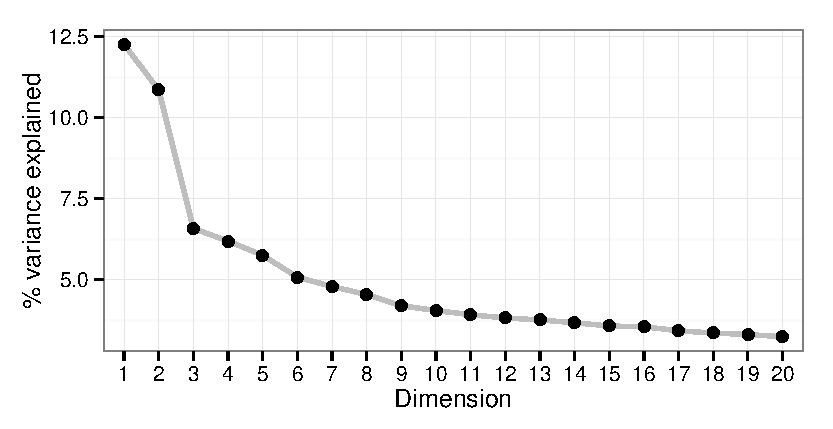
\includegraphics[scale=0.7]{"pictures/demanif-allvarexpl}}

How much variance is explained by adding another dimension?
\begin{itemize}
  \item Remember those $\sigma$s?
\end{itemize}

\end{frame}

\begin{frame}{Common space}

Scaling has notorious comparison problems, mostly due to concerns about 
differential item functioning (DIF).
\begin{itemize}
  \item Is there a 'common space' \parencite{Kluver2009}
  \item Can we construct one? using bridging observations or projection?
\end{itemize}

\end{frame}
\begin{frame}{'Common space'}

\centerline{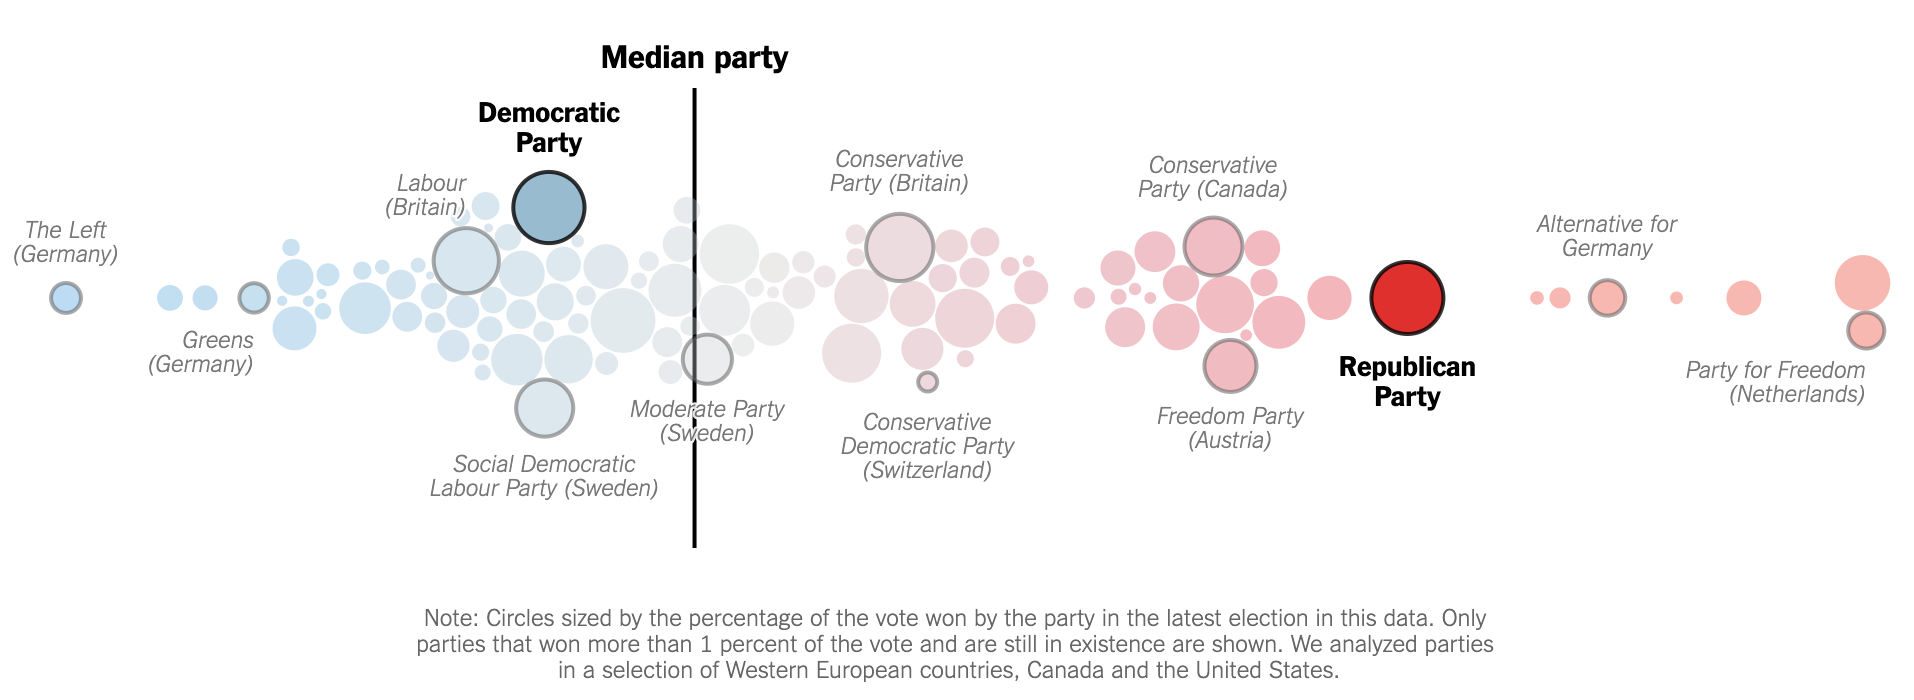
\includegraphics[scale=0.45]{pictures/nyt-parties}}


\end{frame}
\begin{frame}{American parties occupy Germany('s party space)}

\centerline{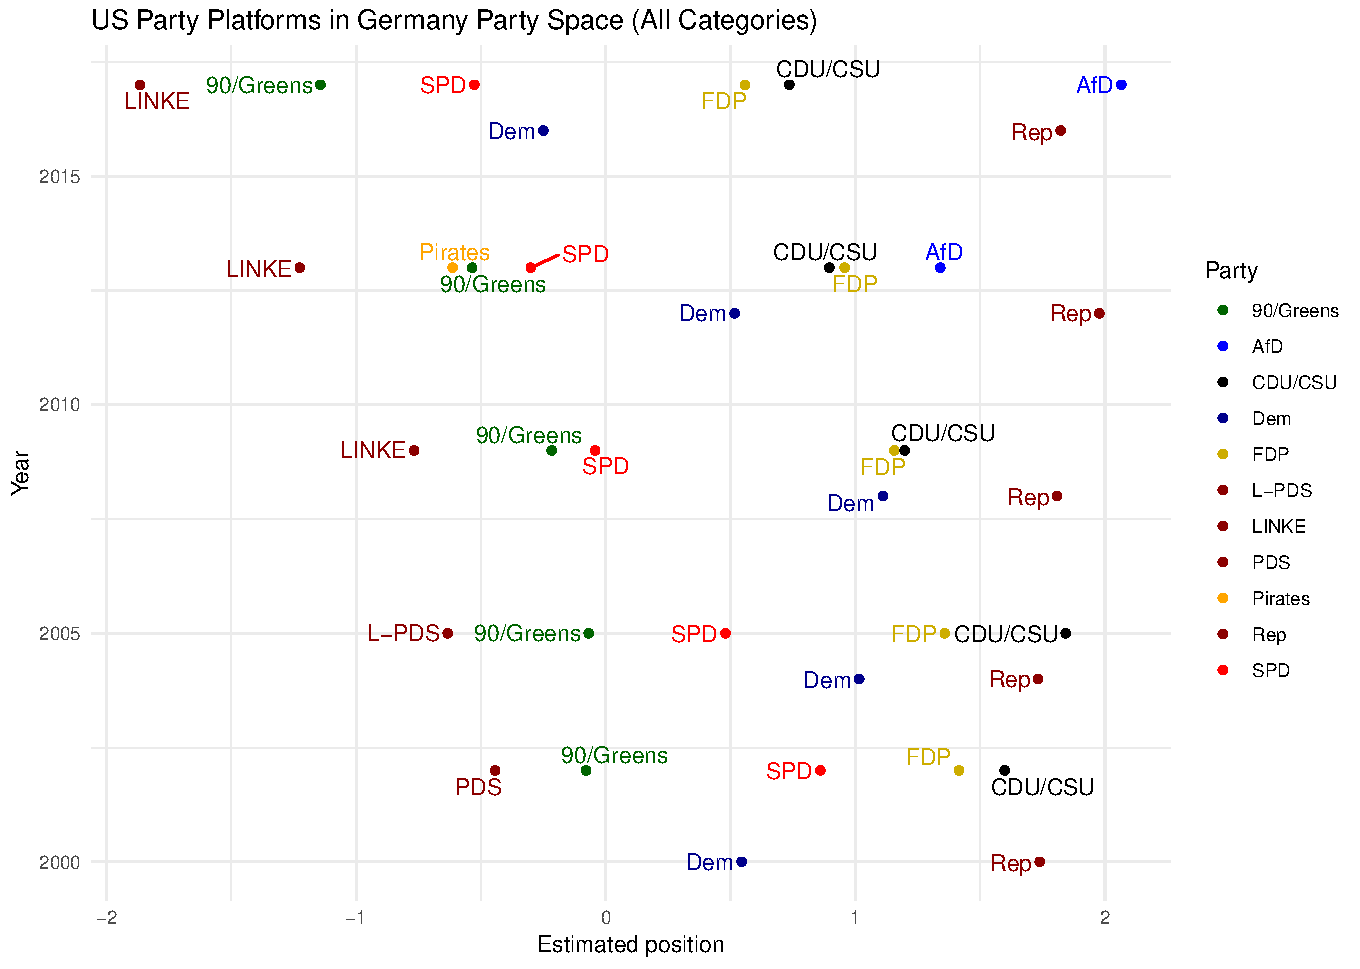
\includegraphics[scale=1]{pictures/cmpcats_us_in_de}}


\end{frame}

%%%%%%%%%%%%%%%%%%%%%%%%%%%%%


\begin{frame}{Scaling several}
\vspace{-1em}
\centerline{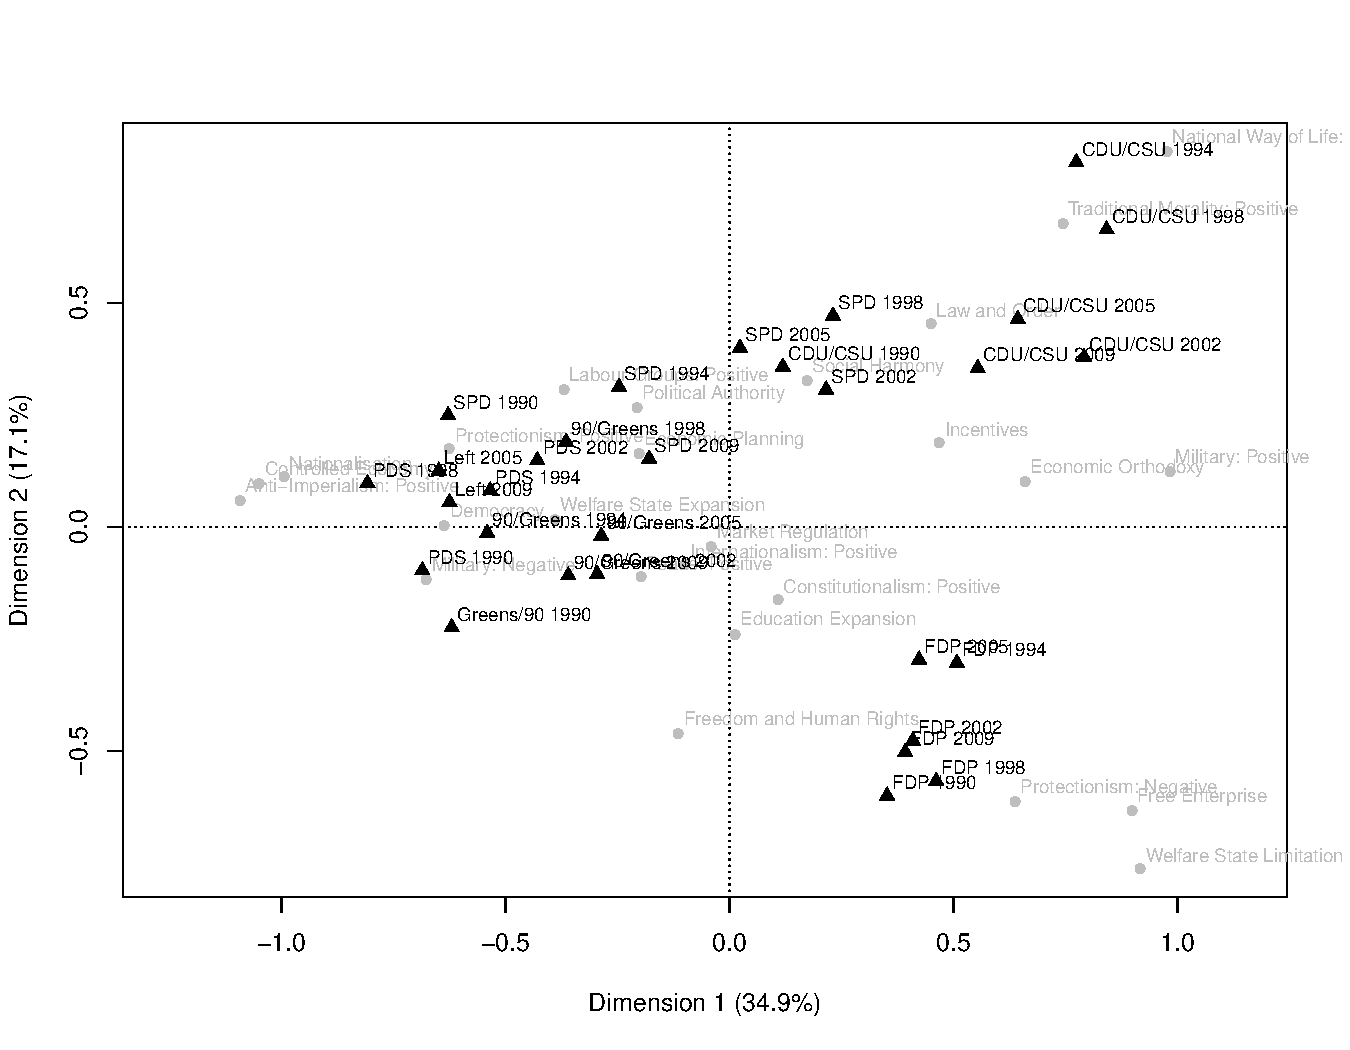
\includegraphics[scale=0.45]{pictures/grey-just-rile}}
Post-1989 German party position from CMP-coded platforms

\end{frame}

\begin{frame}{In each other's space}
\medskip
\centerline{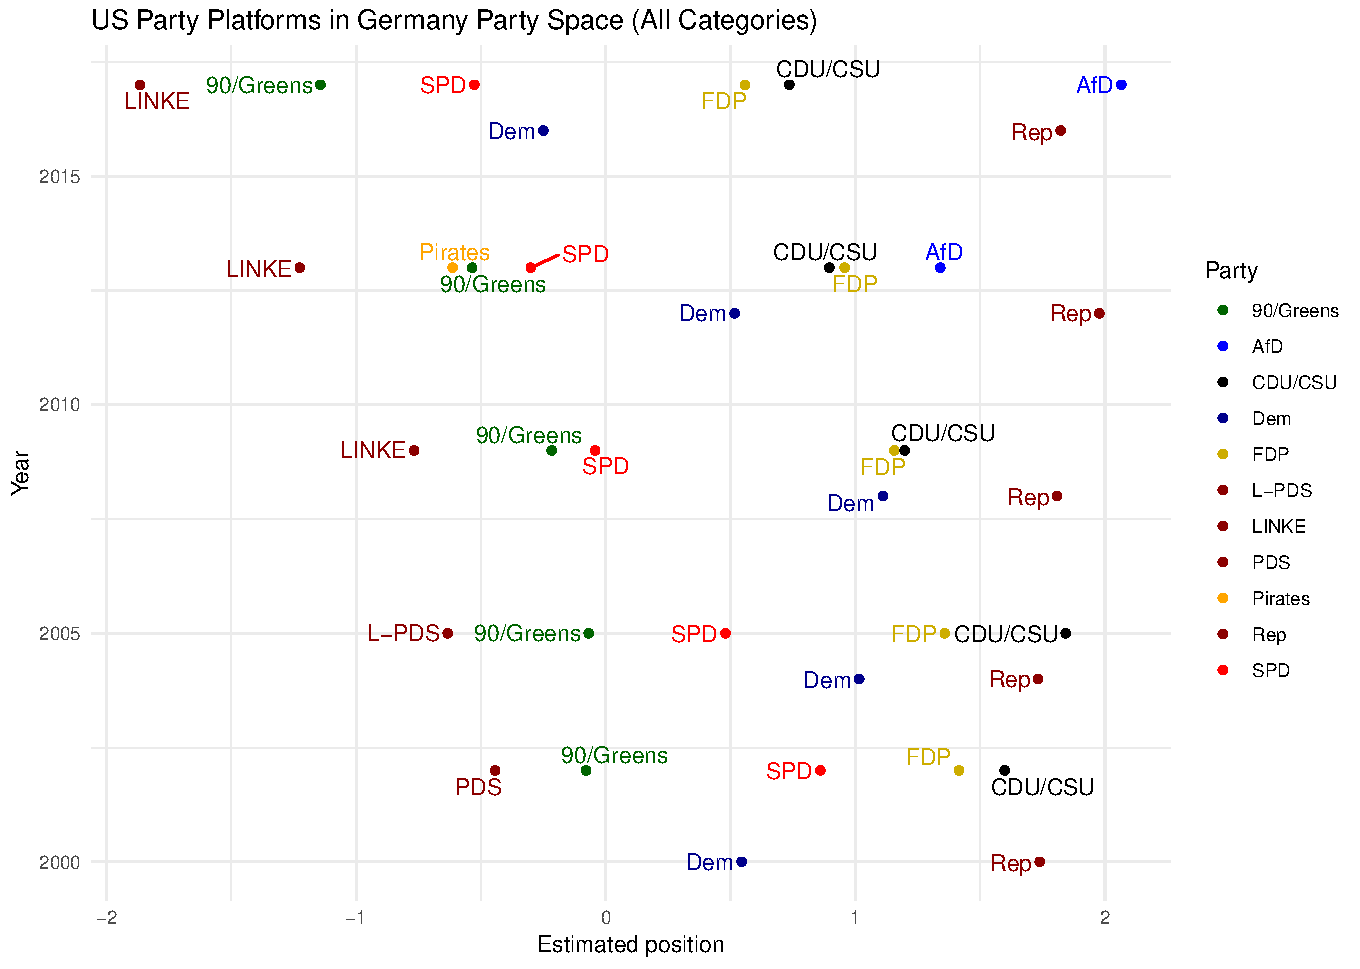
\includegraphics[scale=.35]{pictures/cmpcats_us_in_de}}
Link: \href{https://www.nytimes.com/interactive/2019/06/26/opinion/sunday/republican-platform-far-right.html}{the pretty version at the New York Times}

\end{frame}


%%%

\begin{frame}[allowframebreaks]
\frametitle{References}
\printbibliography	
\end{frame}

\end{document}